\subsection{Das Pol-Nullstellenplot}

In Abbildung \ref{fig:pnp} ist das Pol-Nullstellenplot zu dem System zu sehen. Die x markierten Stellen zeigen die Polstellen an. Dieses System hat keine Nullstellen. Die Polstellen des Systems befinden sich im negativen (0 inkludiert) Teil der reell-wertigen Achse und zeigt somit, dass das System stabil ist.

\begin{figure}[H]
	\centering
	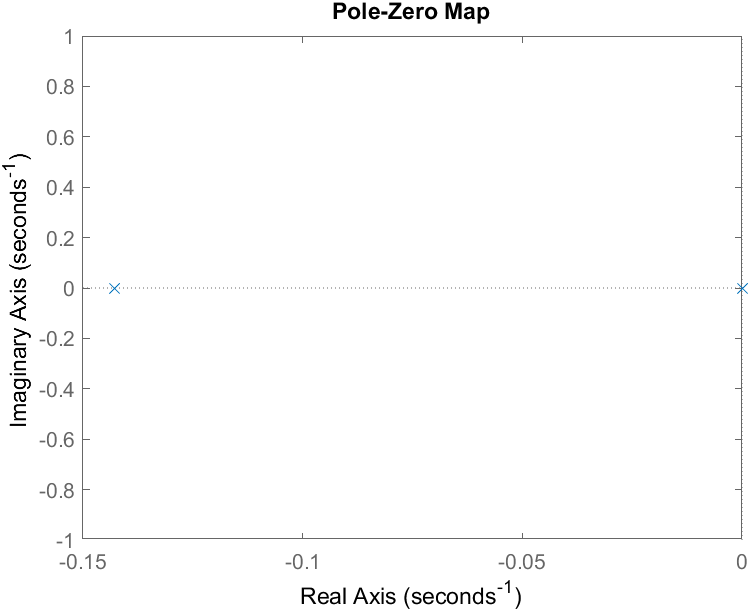
\includegraphics[width=0.8\textwidth]{{diagrams/pol_nullstellenplot.png}}
	\caption[Pol-Nullstellenplot]{Pol-Nullstellenplot}
	\label{fig:pnp}
\end{figure}